\chapter{The triangulation refinement}\label{chap:triangulation}
The purpose of this chapter is to provide an alternative approach to the $\alpha$-shapes methods for determining the boundaries $\partial \mbox{\set{R}{}{}}(\Pi)$ in target PS. 
Our method is based on the triangulation refinement of the source PS explained in Section \ref{chap:PS}.
We have seen that, using the triangulation refinement, more rays close to the boundaries are traced selecting increasingly smaller values for the parameters $\varepsilon_{\variabile{q}_1}^{\textrm{min}}$ and $\varepsilon_{\variabile{p}_1}^{\textrm{min}}$. Once the algorithm stops, only the triangles that are expected to be crossed by a boundary are taken into account. By construction, each of these triangles has two vertices that follow the same path and one vertex that follows another path.
The triangles are ordered in such a way that two of them are neighbors if they have a side in common. Given a path $\Pi$ the corresponding boundary $\partial\mbox{\set{R}{$1$}{}}(\Pi)$ is approximated by those vertices of the triangles which corresponding rays follow path $\Pi$.
The boundaries $\partial \mbox{\set{R}{}{}}(\Pi)$ at the target are given by
\begin{equation}\map{M}{}{}(\partial\mbox{\set{R}{}{}}(\Pi)):\partial\mbox{\set{R}{$1$}{}}(\Pi)\rightarrow\partial\mbox{{R}{}{}}(\Pi),\end{equation}
where $\map{M}{}{}(\partial\mbox{\set{R}{}{}}(\Pi))$ is the restriction of $\map{M}{}{}$, defined in Equation (\ref{eq:map1}), to $\partial\mbox{\set{R}{}{}}(\Pi)$ for every path 
$\Pi$. \\\indent In this chapter we develop a criterion to establish the value of the parameters $\varepsilon_{\variabile{q}_1}^{\textrm{min}}$, $\varepsilon_{\variabile{q}_1}^{\textrm{max}}$, $\varepsilon_{\variabile{p}_1}^{\textrm{min}}$ and $\varepsilon_{\variabile{p}_1}^{\textrm{max}}$ that gives a good approximation of $\partial \mbox{\set{R}{}{}}(\Pi)$.
 Similar to what it was done for selecting $\alpha$ in the $\alpha$-shapes procedure, 
the triangulation parameters are selected using the \'{e}tendue conservation in PS. The core of our approach is the following.\\
\indent The \'{e}tendue $U_1$ at the source PS \set{S}{}{} related to all the rays that arrive at the target is calculated. If all the rays emitted by the source are received by the target, $U_1$ can be easily determined by using Equation (\ref{eq:etenduesource}), otherwise Equation (\ref{eq:etenduesumsource}) needs to be computed. 
\\ \indent The \'{e}tendue $U_{\textrm{t}}$ at the target PS \set{T}{}{} is computed using Equations (\ref{eq:etendueintegraltarget}) and (\ref{eq:etenduetarg1}).
To calculate the integral in Equation (\ref{eq:etenduetarg1}), the triangulation refinement method is applied to the regions $\mbox{\set{R}{}{}}(\Pi)$ for a range of values of $\varepsilon_{\variabile{q}_1}^{\textrm{max}}$ and for a fixed value of $\varepsilon_{\variabile{q}_1}^{\textrm{min}}$. The parameters along the $\variabile{q}$-axis are scaled as $\varepsilon_{\variabile{p}_1}^{\textrm{max}} = \varepsilon_{\variabile{q}_1}^{\textrm{max}}/w$ and 
$\varepsilon_{\variabile{p}_1}^{\textrm{min}}  = \varepsilon_{\variabile{q}_1}^{\textrm{min}}/w$ with 
$w = (\variabile{p}_1^{\textrm{max}}-\variabile{p}_1^{\textrm{min}})/(\variabile{q}_1^{\textrm{max}}-\variabile{q}_1^{\textrm{min}})$ where 
$\variabile{p}_1^{\textrm{min}}$ and $\variabile{p}_1^{\textrm{max}}$ are the minimum and the maximum $\variabile{p}$-coordinate in \set{S}{}{}, respectively, and 
$\variabile{q}_1^{\textrm{min}}$ and $\variabile{q}_1^{\textrm{max}}$ are the minimum and the maximum $\variabile{q}$-coordinate in \set{S}{}{}, respectively.
An approximation of the boundaries $\partial\mbox{\set{R}{}{}}(\Pi)$ is obtained for each of those parameters values.
Then, the intersection points $(\variabile{q}^{\variabile{i}}( \Pi, \variabile{p}), \Pi)_{\variabile{i} = 1, \cdots, \variabile{r}}$ between $\partial\mbox{\set{R}{}{}}(\Pi)$
and the horizontal line $\variabile{p}~=~ const$ are calculated for each path $\Pi$, and for $\variabile{p}~\in~[-1,1]$. Ordering their $\variabile{q}$-coordinates in ascending order, the integral in Equation (\ref{eq:etenduetarg1}) is computed.
Changing the values of the parameters, different approximations of $\partial\mbox{\set{R}{}{}}(\Pi)$ are found and, consequently, different values of $U_{\textrm{t}}$
\\ \indent In order to use the parameters that give a good accuracy of the target photometric variables, the difference $\Delta U = U_1-U_{\textrm{t}}$ is calculated for every value of $U_{\textrm{t}}$ found. The values of the parameters that give the smaller distance $\Delta$ define the more accurate triangulation at source PS \set{S}{}{}. Hence, these values are chosen for the computation of the target photometric variables. \\\indent
The method explained above is tested for several optical systems. The results are presented next.
\section{The two-faceted cup}
In this paragraph we apply the triangulation refinement in PS to the two-faceted cup described in Chapter \ref{chap:raytracing} and depicted in Figure \ref{fig:cup}. 
We start tracing rays inside the system using PS ray tracing as explained in Chapter \ref{chap:PS}. To avoid rays parallet to the source and that leave the endpoints, we consider rays with initial direction $\variabile{p}_1\in[-1+10^{-6},1-10^{-6}]$ and initial position $\variabile{q}\in[-2+10^{-12}, 2-10^{-12}]$. In order to define a stopping criterion for the triangulation, we apply \'{e}tendue conservation. Since the two-faceted cup is formed by only reflective lines and its target is adjacent to the left and the right reflector (it is located exactly at the top of the system),  all the rays emitted by the source arrive to the target. Thus, 
\begin{equation}U_1 = U\approx 8, \end{equation}
where the second equality follows from Equation (\ref{eq:etenduesource}) with $\n_1\sin(\myangle_1^{\textrm{max}})=\variabile{p}_1^\textrm{max}=1-10^{-6}$ and $\variabile{a}=2+10^{-12}$.\\
To define a stopping criterion for the triangulation at the source PS and determine how many rays are needed to acieve a good accuracy of the target intensity, we compute the target \'{e}tendue $U_{\textrm{t}}$ and we compare the approximated value with the exact value at the source $U_1$. 
To this purpose, ray tracing in PS is implemented for a range of values of $\varepsilon_{\variabile{q}_1}^{\textrm{min}}$, $\varepsilon_{\variabile{q}_1}^{\textrm{max}}=1$, $\varepsilon_{\variabile{p}_1}^{\textrm{max}} = \varepsilon_{\variabile{q}_1}^{\textrm{max}}/w$, and $\varepsilon_{\variabile{p}_1}^{\textrm{min}}= \varepsilon_{\variabile{q}_1}^{\textrm{min}}/w$ where $w = (\variabile{p}_1^{\textrm{max}}-\variabile{p}_1^{\textrm{min}})/(\variabile{q}_1^{\textrm{max}}-\variabile{q}_1^{\textrm{min}})\approx2$. 
The approximated boundaries are computed for each of these values joining the vertices of those triangles crossed by a boundary that follow the same path $\Pi$. 
In Figure \ref{fig:boundaries_cup} we show, with the black lines, the boundaries of \set{R}{$1$}{}$(\Pi)$ and \set{R}{}{}$(\Pi)$ found for two different values of $\varepsilon_{\variabile{q}_1}^{\textrm{min}}$. Note that, decreasing $\varepsilon_{\variabile{q}_1}^{\textrm{min}}$, the number of rays increases. 
\begin{figure}[h!]
\centering
\begin{subfigure}{.45\textwidth}
  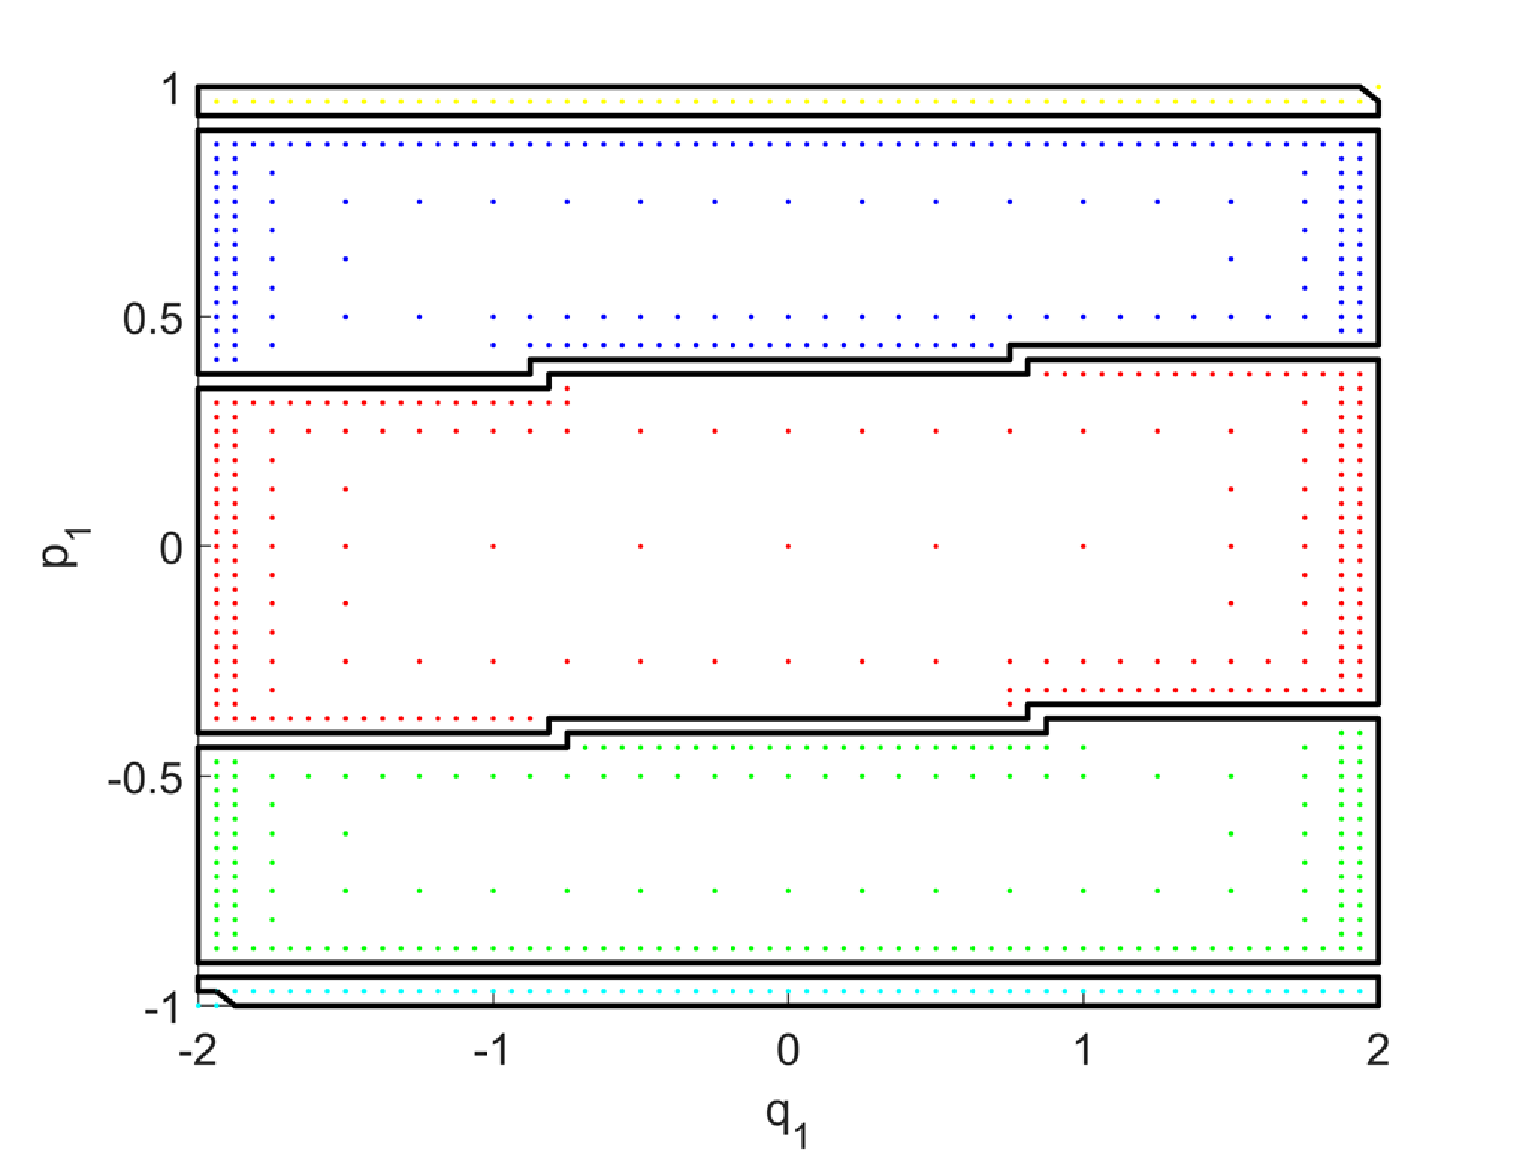
\includegraphics[width=\textwidth]{boundaries_source_triangles2}
 \caption{The black lines are the boundaries at \set{S}{}{}. $1500$ rays are traced using the triangulation refinement with $\varepsilon_{\variabile{q}_1}^{\textrm{min}}=0.1$. }
  \label{fig:boundary_s2}
\end{subfigure}%
\begin{subfigure}{.45\textwidth}
  
\includegraphics[width=\textwidth]{boundaries_target_triangles2}
  \caption{The black lines are the boundaries at \set{T}{}{}. $1500$ rays are traced using the triangulation refinement with $\varepsilon_{\variabile{q}_1}^{\textrm{min}}=0.1$.} %$U_{\textrm{t}}\approx7.468.$}
  \label{fig:boundaries_t2}
\end{subfigure} %
\begin{subfigure}{.45\textwidth}
  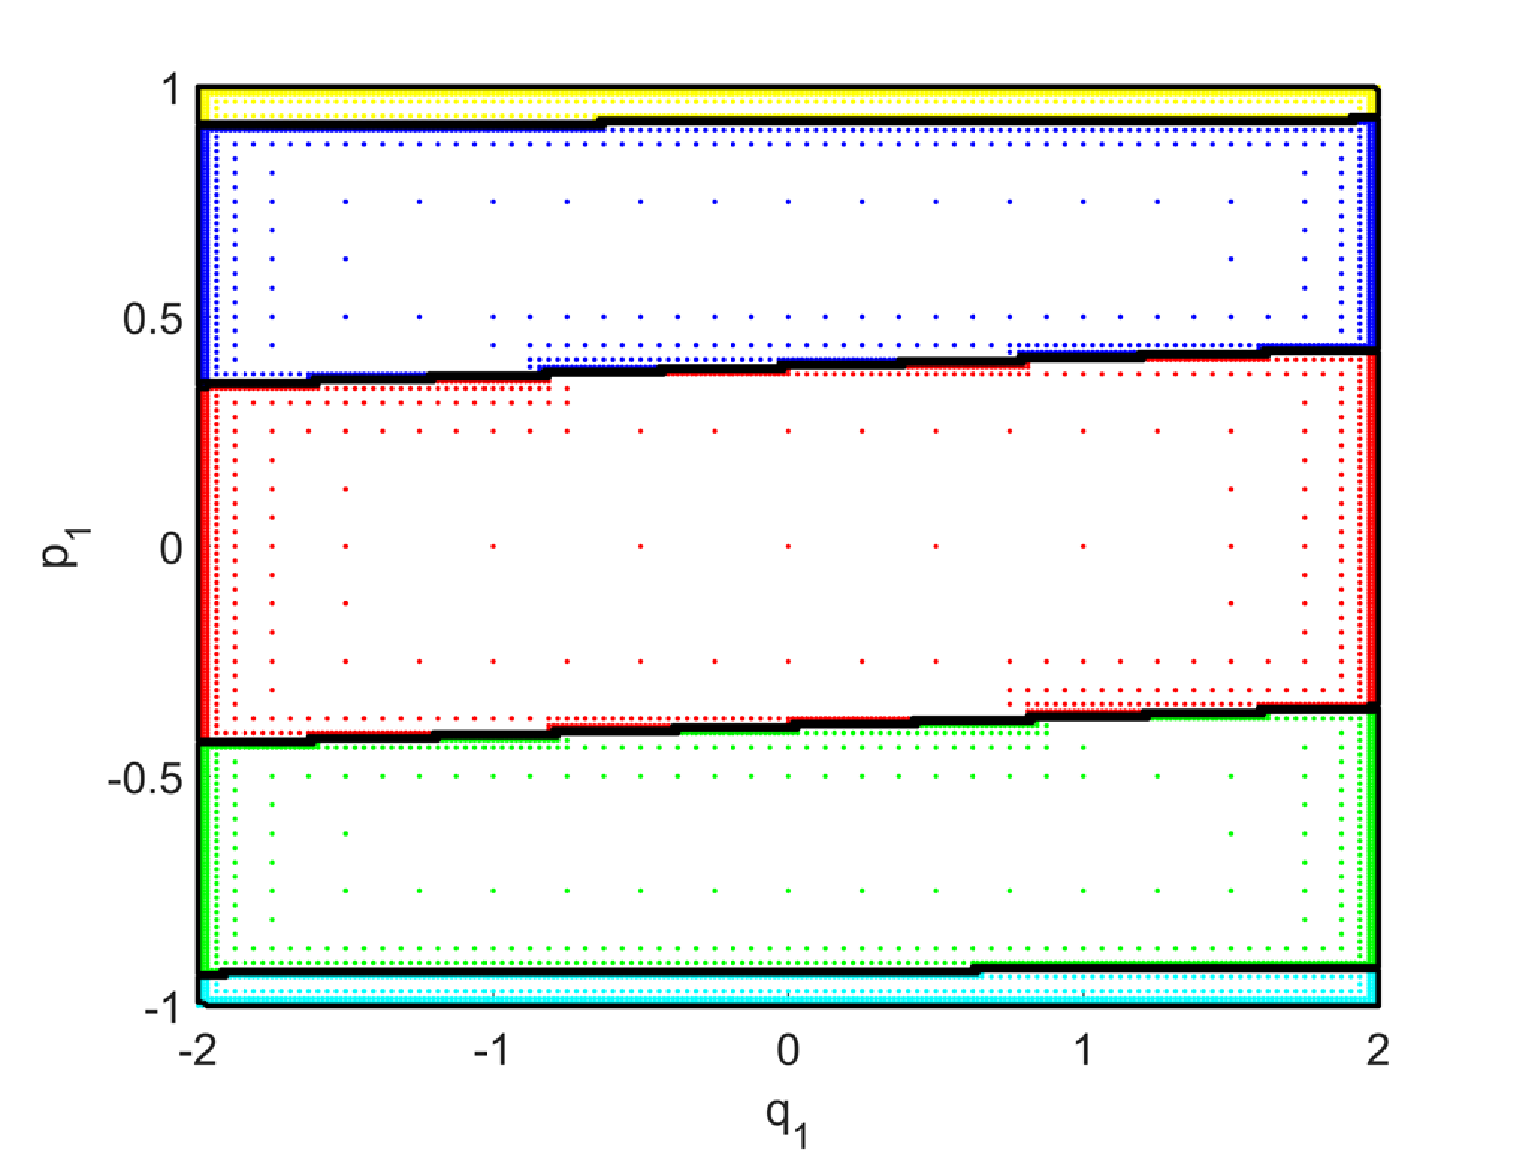
\includegraphics[width = \textwidth]{boundaries_source_triangles1}
  \caption{The black lines are the boundaries at \set{S}{}{}. $7500$ rays are traced using the triangulation refinement with $\varepsilon_{\variabile{q}_1}^{\textrm{min}}=0.05/2$.}
  \label{fig:boundaries_s1}
\end{subfigure}%
\begin{subfigure}{.45\textwidth}
  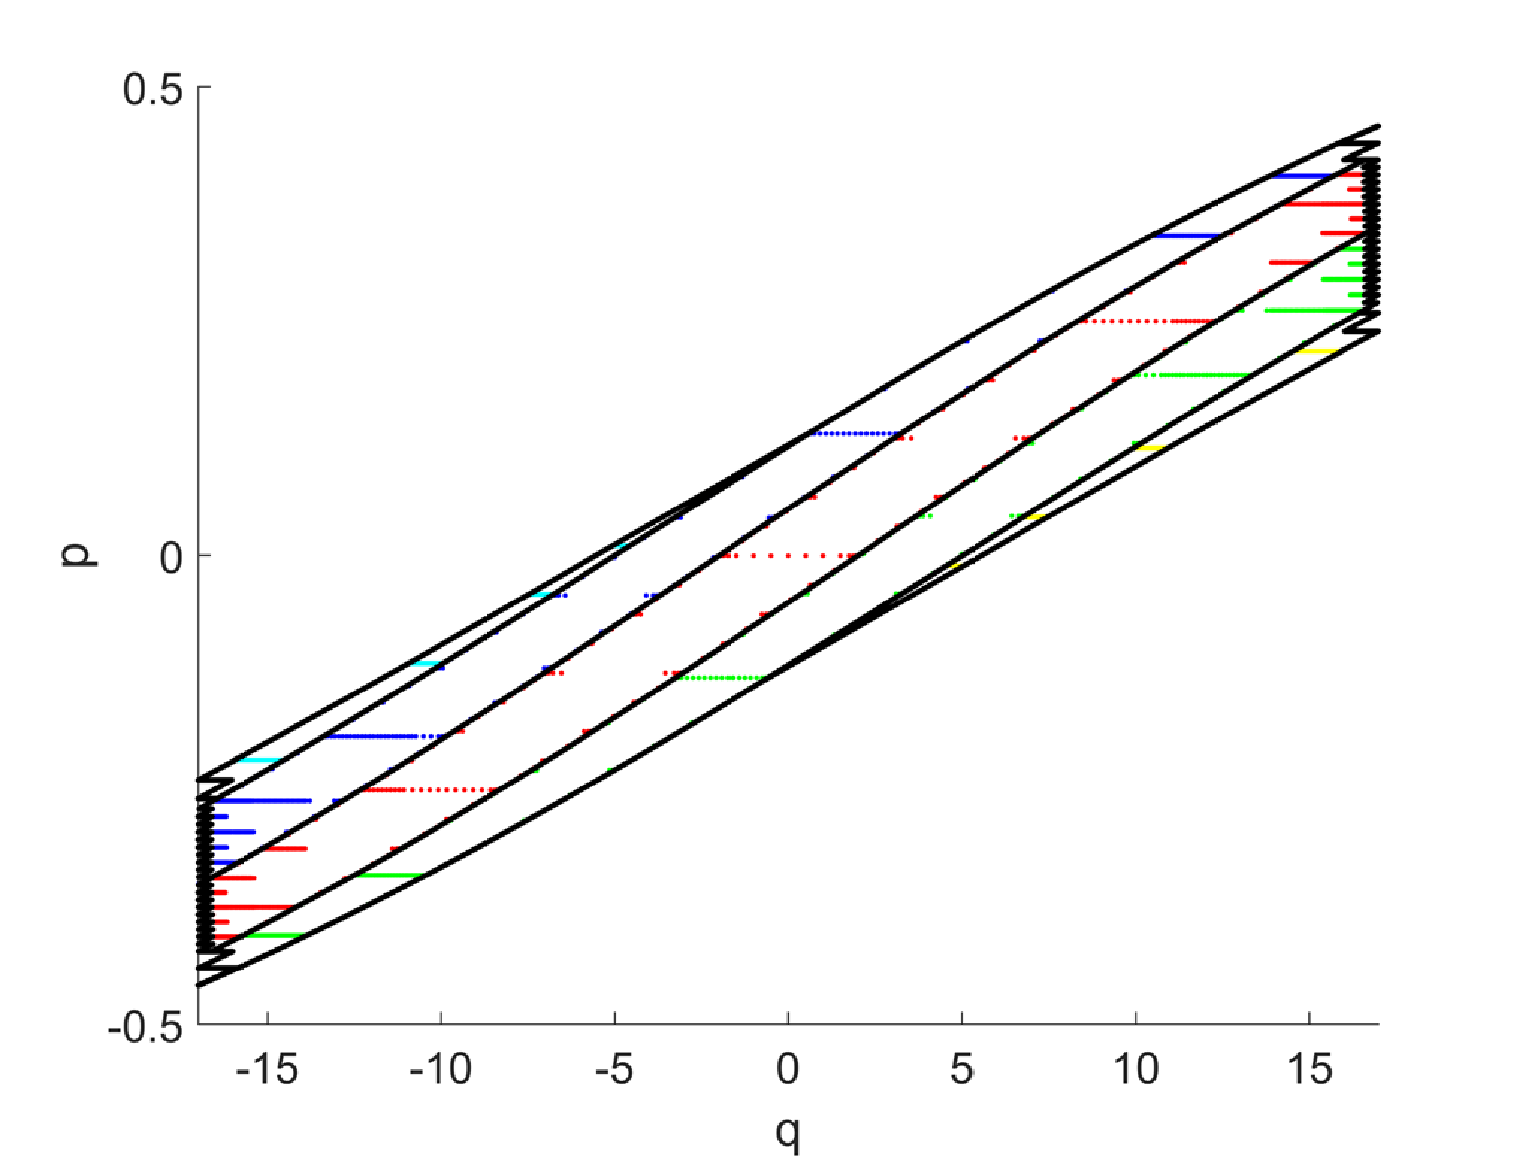
\includegraphics[width=\textwidth]{boundaries_target_triangles1}
 \caption{The black lines are the boundaries at \set{T}{}{}. $7500$ rays are traced using the triangulation refinement with $\varepsilon_{\variabile{q}_1}^{\textrm{min}}=0.05/2$.} %$U_{\textrm{t}}\approx7.867.$}
  \label{fig:boundaries_t1}
\end{subfigure}
\caption{\textbf{Boundaries at \set{S}{}{} and \set{T}{}{} of the two-faceted cup.} The approximated boundaries are computed using the triangulation refinement with two different values of $\varepsilon_{\variabile{q}_1}^{\textrm{max}}$.}
\label{fig:boundaries_cup}
\end{figure} 
In order to understand which value of  $\varepsilon_{\variabile{q}_1}^{\textrm{min}}$ gives the best approximation of the boundaries and, consequently, of the target photometric variable, we calculate $U_{\textrm{t}}$ for the every set of rays traced using Equation (\ref{eq:etenduetarg1}). Then the difference 
\begin{equation}\label{eq:delta} \Delta U = U_1-U_{\textrm{t}} 
\end{equation} is found.
An accurate approximation of $U_{\textrm{t}}$ gives a small value of $\Delta U$. 
For instance, for the two set of rays depicted Figures \ref{fig:boundaries_cup} we found $\Delta U \approx 0.53 $ for $\varepsilon_{\variabile{q}_1}^{\textrm{min}} = 0.1$ and $\Delta U \approx 0.13 $ for $\varepsilon_{\variabile{q}_1}^{\textrm{min}} = 0.05/2$. This give the insight that the boundaries computation obtained using $\varepsilon_{\variabile{q}_1}^{\textrm{min}} = 0.05/2$ is more accurate.
\\ \indent In Figure \ref{fig:etendue_cup} we show with the blue line how the target \'{e}tendue varies as a function of the parameter $\varepsilon_{\variabile{q}_1}^{\textrm{min}}$ where the other parameter have always a fixed value. The exact \'{e}tendue $U=8$ is depicted with the red line and it is computed using Equation (\ref{eq:etenduetarg1}). By decreasing $\varepsilon_{\variabile{q}_1}^{\textrm{min}}$ an increase of $U_{\textrm{t}}$ is observed. Furthermore, by construction, $U_{\textrm{t}}$ is always underestimated because the approximated boundaries are found joining the vertices of the \textit{boundaries triangles} which are \textit{inside} the regions \set{R}{}{}$(\Pi)$. Where the \textit{boundary triangles} are those crossed by a boundary.
 \begin{figure}[h!]
  \center
  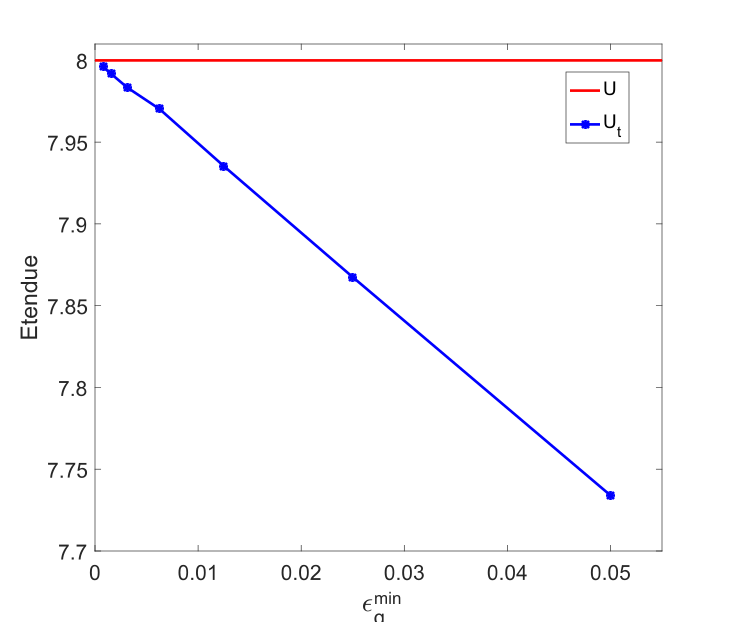
\includegraphics[width= 7cm]{etendue_cup_epsilon}
  \caption{\textbf{Etendue for the two faceted cup.} The total \'{e}tendue as an area in PS is depicted with the red line. The approximated \'{e}tendue for a range of values of 
$\varepsilon_{\variabile{q}_1}^{\textrm{min}}$ is shown with the blue line.}
  \label{fig:etendue_cup}
\end{figure}
Referring as Figure \ref{fig:etendue_cup}, the best approximation of $U_{\textrm{t}}$ is obtained tracing around $1.2 \cdot 10^5$ rays using PS ray tracing with parameters $\varepsilon_{\variabile{q}_1}^{\textrm{min}}=0.8\cdot 10^{-4}$, $\varepsilon_{\variabile{q}_1}^{\textrm{max}}=1$, $\varepsilon_{\variabile{p}_1}^{\textrm{min}}=\varepsilon_{\variabile{q}_1}^{\textrm{min}}/2$ and $\varepsilon_{\variabile{q}_1}^{\textrm{max}}= \varepsilon_{\variabile{q}_1}^{\textrm{max}}/2$. 
%The approximated boundaries $\partial$\set{R}{}{}$(\Pi)$ corresponding to those parameters are shown in Figure \ref{fig:best_boundaries_cup}.
\\ \indent The PS intensity $\hat{I}_{PS}$ with $1.2 \cdot 10^5$ rays is calculated using Equation (\ref{eta2}). The intensity profile is shown in Figure \ref{fig:intensity_cup_triangulation} with the red line. In the same graph we show the reference intensity $\hat{I}_{\textrm{ref}}$ with the dotted blue line. For the two-faceted cup the reference intensity is actually the exact intensity ($\hat{I}_{\textrm{ref}}= \hat{I}_{\textrm{exact}}$). 
 \begin{figure}[h!]
  \center
  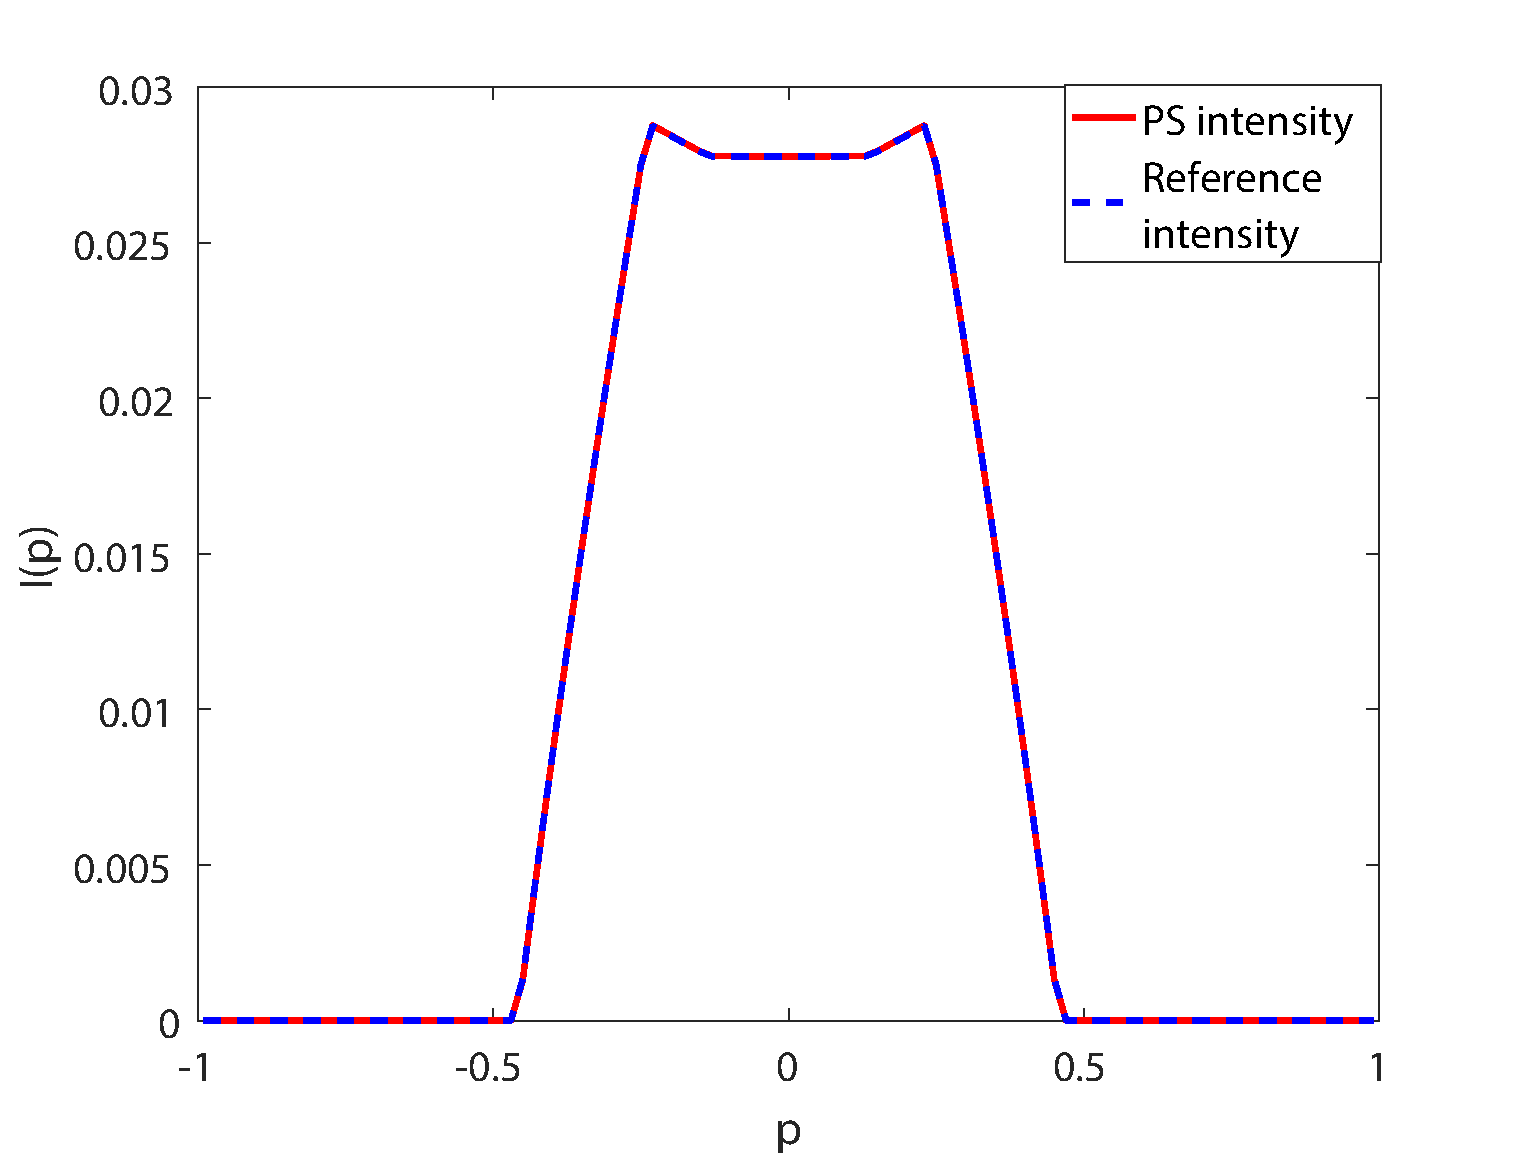
\includegraphics[width= 7cm]{intensity_cup_triangulation}
  \caption{\textbf{Intensity profile at the target of the two faceted cup.} The reference intensity is an analytic intensity. The PS intensity is computed using the triangulation refinement with $\varepsilon_{\variabile{q}_1}^{\textrm{min}}=0.8\cdot 10^{-4}$, $\varepsilon_{\variabile{q}_1}^{\textrm{max}}=1$, $\varepsilon_{\variabile{p}_1}^{\textrm{min}}=\varepsilon_{\variabile{q}_1}^{\textrm{min}}/2$ and $\varepsilon_{\variabile{p}_1}^{\textrm{max}}= \varepsilon_{\variabile{q}_1}^{\textrm{max}}/2$. Around $1.2 \cdot 10^5$ rays are traced.}
  \label{fig:intensity_cup_triangulation}
\end{figure}
\\ \indent 
Finally, we compare PS ray tracing with both MC and QMC ray tracing by computing the error between the approximated intensities $\hat{I}_{\textrm{A}}  (\textrm{A}= \textrm{MC}, \textrm{QMC}, \textrm{PS})$ and the exact intensity $\hat{I}_{\textrm{ref}}$ defined in Equation (\ref{eq:error}) with $\nbin = 100$. The results are shown in Figure \ref{fig:error_cup_triangulation} where MC, QMC and PS intensity are depicted with the green, blue and red line, respectively.
 \begin{figure}[h]
  \center
  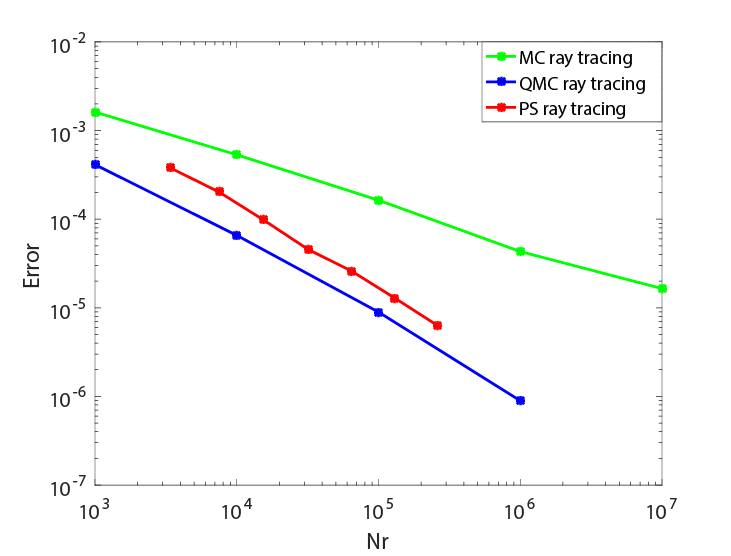
\includegraphics[width= 7cm]{error_cup_triangulation.png}
  \caption{\textbf{Error plot for the two faceted cup.} The errors between the approximated intensities $\hat{I}_{\textrm{A}} (\textrm{A}= \textrm{MC}, \textrm{QMC}, \textrm{PS})$ and the exact intensity $\hat{I}_{\textrm{exact}}$ are shown in a logarithmic scale. Using PS ray tracing far less rays need to be traced compared to MC ray tracing but still more rays than QMC ray tracing are needed.}
  \label{fig:error_cup_triangulation}
\end{figure}
The results for the two-faceted cup show that using PS and the triangulation refinement for the boundaries computation requires tracing far less rays compared to MC ray tracing.
An error comparison between QMC ray tracing and PS ray tracing shows that more rays are needed in PS. This can be due to the fact that with the triangulation refinement we always underestimate the value of the \'{e}tendue at the target. Although, the shape of all the regions \set{R}{}{}$(\Pi)$ are very smooth, their boundaries are difficult at the edge of the target phase space \set{T}{}{} to approximate by triangles. With the triangulation refinement, as far as is fine the triangulation, the vertical and straight lines at the edge of \set{T}{}{} are always approximate by a broken line. On the contrary, since the two-faceted cup is a very simple system, QMC ray tracing does not requires a huge number of rays to obtain the desired accuracy. Nevertheless, PS ray tracing has a big advantage compared to QMC ray tracing. Indeed, as we have seen in Chapter \ref{chap:raytracing}, MC and QMC ray tracing are binning procedure. Therefore, the MC and QMC intensities are given by the average over every bin and the error also depends on the number of bins. This part of the error is not included in the results provided in Figure \ref{fig:error_cup_triangulation} as there we have fixed the number of bins $\nbin = 100$. % according to Equations \ref{} \ref{}
PS ray tracing gives a pointwise intensity along all the possible directions. In the simulations shown in this thesis we always compute the average PS intensity. This is needed to give a fair comparison of PS ray tracing with MC and QMC ray tracing. Note that no error related to the number of bins is included in the PS method. \\ \indent
In order to investigate in more details the PS ray tracing performances, we test the procedure for more complicated systems. In the next paragraph we present the results for a TIR-collimator. 
\section{A TIR-collimator}
In this section we provide the results of PS ray tracing for a TIR-collimator, using the triangulation refinement to compute the boundaries $\partial$\set{R}{}{}$(\Pi)$ in target PS. In particular, we consider the TIR-collimator depicted in Figure \ref{fig:analyticlens}. Since this system is located in two different media (air and glass), also refraction law plays a role in the ray tracing procedure. We implement PS ray tracing for the TIR-collimator gradually increasing the number of rays, i.e. gradually decreasing the values of the parameters $\varepsilon_{\variabile{q}_1}^{\textrm{min}}, \varepsilon_{\variabile{q}_1}^{\textrm{max}}, \varepsilon_{\variabile{p}_1}^{\textrm{min}}$ and $\varepsilon_{\variabile{p}_1}^{\textrm{max}}$ in the triangulation. In order to trace more rays close to the boundaries, we decide to vary only the value of $\varepsilon_{\variabile{q}_1}^{\textrm{min}}$ and $ \varepsilon_{\variabile{p}_1}^{\textrm{min}}$ which determine the number of triangles close to the boundaries and we hold fixed the values of $ \varepsilon_{\variabile{q}_1}^{\textrm{max}}$ and $ \varepsilon_{\variabile{p}_1}^{\textrm{max}}$ as they are responsible of the number of rays inside the regions \set{R}{}{}$(\Pi)$. Every ray traced has initial position coordinate $\variabile{q}_1\in[-\variabile{a}, \variabile{a}]$ with $\variabile{a}=2$ and the initial direction coordinate $\variabile{p}_1=[-1.1]$. Therefore, the source PS of the TIR-collimator is the rectangular \set{S}{}{}$= [-2, 2] \times [-1, 1]$. The parameters $\varepsilon_{\variabile{p}_1}^{\textrm{min}}$ and $\varepsilon_{\variabile{p}_1}^{\textrm{max}}$ are scaled as follows:
\begin{equation}
\begin{aligned}
& w = \frac{\variabile{p}_1^{\textrm{max}}-\variabile{p}_1^{\textrm{min}}}{\variabile{q}_1^{\textrm{max}}-\variabile{q}_1^{\textrm{min}}}=2,\\
&\varepsilon_{\variabile{p}_1}^{\textrm{min}}= \frac{\varepsilon_{\variabile{q}_1}^{\textrm{min}}}{w}, \\
&\varepsilon_{\variabile{p}_1}^{\textrm{max}}= \frac{\varepsilon_{\variabile{q}_1}^{\textrm{max}}}{w}.
\end{aligned}
\end{equation}
\\ \indent To determine the triangulation refinement that gives a good approximation of the target intensity we compare $U_1$ (source \'{e}tendue) to $U_{\textrm{t}}$ (target \'{e}tendue) and use \'{e}tendue conservation property. Now, not all light emitted by the source of the TIR-collimator arrives at its target. Indeed, using PS ray tracing $\npath=7$ different paths $(\Pi_\lineai)_{\lineai=1, \cdots, \npath}$ are found but only five of them are paths from the source (line $1$) to the target (line $12$), see Section \ref{sec:results-Tir-alpha}. Thus, we need to remove from the total area of \set{S}{}{} those parts occupied by the rays that arrive at some others detectors and not at the target. % white areas in figure...
The source PS is given by:
\begin{equation}
U_1 = 8-2A_T\approx 7.77.
\end{equation}
The target \'{e}tendue $U_{\textrm{t}}$ is obtained from Equation (\ref{eq:etenduetarg}) for a range of values of $\varepsilon_{\variabile{q}_1}^{\textrm{min}}$ and with $\varepsilon_{\variabile{q}_1}^{\textrm{max}}=1$ fixed. Likewise, the two-faceted cup, the boundaries $\partial$\set{R}{}{}$(\Pi)$ are found for every value of $\varepsilon_{\variabile{q}_1}^{\textrm{min}}$, and $U_{\textrm{t}}$ is calculated for each of these boundaries. 
The results shown in Figure \ref{fig:etendue_tir_triangulation} give the \'{e}tendue plot a function of $\varepsilon_{\variabile{q}_{1}^{\textrm{min}}}$.
%\begin{table}[h!] \label{tab:etendue_tir_triangulatio}
%\centering
%\caption{\bf Etendue as a function of $\nrays$ and $\varepsilon_{\variabile{q}_1}^{\textrm{min}} $}
%\begin{tabular}{lll}
% \hline  \nrays\;  & $\varepsilon_{\variabile{q}_1}^{\textrm{min}} $ \; & \'{e}tendue  \\
%  \hline 
% $3\,547$ & $0.05$  & $7.50$  \\
%$8\,055$  & $0.025$   & $7.61$   \\
%$17\,300$  & $0.125$  & $7.69$ \\
% $38\,300$  & $6.3\cdot 10^{-3}$   & $7.73$  \\
% $79\,600$ & $3.1\cdot 10^{-3}$   & $7.75$  \\
%$162\,300$ & $1.6\cdot 10^{-3}$  & $7.76$  \\ 
%\hline
% \end{tabular}
% \label{tab:etendue_tir_triangulation}
% \end{table}
 \begin{figure}[h!]
  \center
  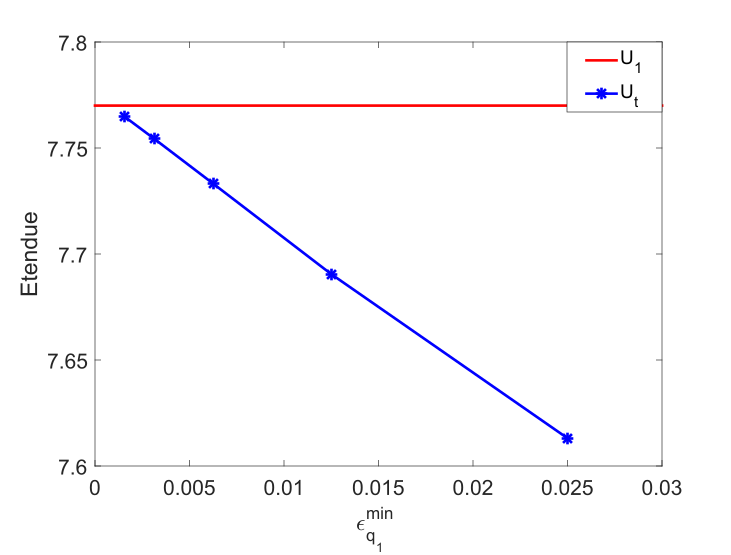
\includegraphics[width= 7cm]{etendue_tir_triangulation}
  \caption{\textbf{Etendue of the TIR-collimator.} A comparison between $U_1$ and $U_{\textrm{t}}$ shows that by decreasing the value of $\varepsilon_{\variabile{q}_{1}^{\textrm{min}}}$, $\Delta U= U_1-U_{\textrm{t}}$ decreases.}
  \label{fig:etendue_tir_triangulation}
\end{figure}
\\ \indent The boundaries $\partial\mbox{\set{R}{$1$}{}}(\Pi_{\lineai})$ and $\partial\mbox{\set{R}{}{}}(\Pi_{\lineai})$ with $\lineai = \{1, \cdots, 5\}$ computed using the triangulation refinement with 
$\varepsilon_{\variabile{q}_1}^{\textrm{min}}=1.6\cdot 10^{-3}$ are shown in Figure \ref{fig:boundaries_TIR_triangulation} with the black lines. 
 \begin{figure}[ht]
  \center
  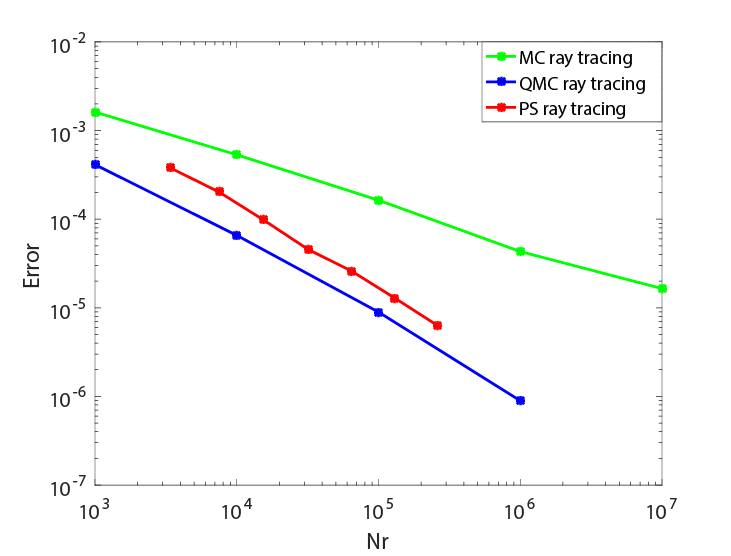
\includegraphics[width= 7cm]{error_cup_triangulation.png}
  \caption{\textbf{Boundaries at \set{S}{}{} and \set{T}{}{} of the TIR-collimator} The black lines show the boundaries found using $\varepsilon_{\variabile{q}_1}^{\textrm{min}}=1.6\cdot 10^{-3}$ in the triangulation refinement of the source PS..}
  \label{fig:boundaries_TIR_triangulation}
\end{figure}
Around $1.62 \cdot 10^5$ rays are traced using the triangulation refinement in PS with $\varepsilon_{\variabile{q}_1}^{\textrm{min}}=1.6\cdot 10^{-3}, \varepsilon_{\variabile{q}_1}^{\textrm{max}}=1, \varepsilon_{\variabile{p}_1}^{\textrm{min}}=\varepsilon_{\variabile{q}_1}^{\textrm{min}}/2$ and $\varepsilon_{\variabile{p}_1}^{\textrm{max}} = \varepsilon_{\variabile{q}_1}^{\textrm{max}}/2$. \\ \indent 
The target PS intensity $\hat{I}_{\textrm{PS}}$ is found for those parameters and it is compared with a reference intensity $\hat{I}_{\textrm{ref}}$ which is given by QMC ray tracing with $10^7$ rays (as the exact intensity for the TIR-collimator is unknown). The profile of the two intensities is given in Figure \ref{fig:intensity_tir_triangulation}. 
The difference between the two intensity profiles is not discernible by eye.
 \begin{figure}[ht]
  \center
  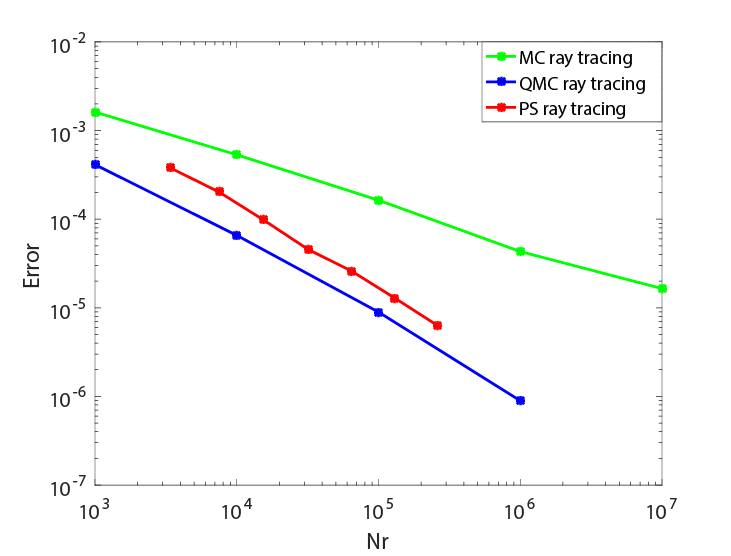
\includegraphics[width= 7cm]{error_cup_triangulation.png}
  \caption{\textbf{Target intensity for the TIR-collimator.} The PS intensity $\hat{I}_{\textrm{PS}}$ is computed using PS ray tracing with around $1.62\cdot 10^5$ rays. The reference intensity $\hat{I}_{\textrm{ref}}$ is obtained by QMC ray tracing with $10^7$ rays.}
  \label{fig:intensity_tir_triangulation}
\end{figure}
\\ \indent
To validate our method, PS ray tracing is compared to both MC and QMC ray tracing. The error between the approximated intensities $\hat{I}_{\textrm{A}} (\textrm{A}=\textrm{QMC}, \textrm{MC}, \textrm{PS})$ and the reference intensity $\hat{I}_{\textrm{ref}}$ as a function of the number of rays traced is calculated. The error plot is shown in Figure \ref{fig:error_tir_triangulation} where the green line shows the MC, QMC and PS convergences are shown with the green, the blue and the red line, respectively. 
 \begin{figure}[ht]
  \center
  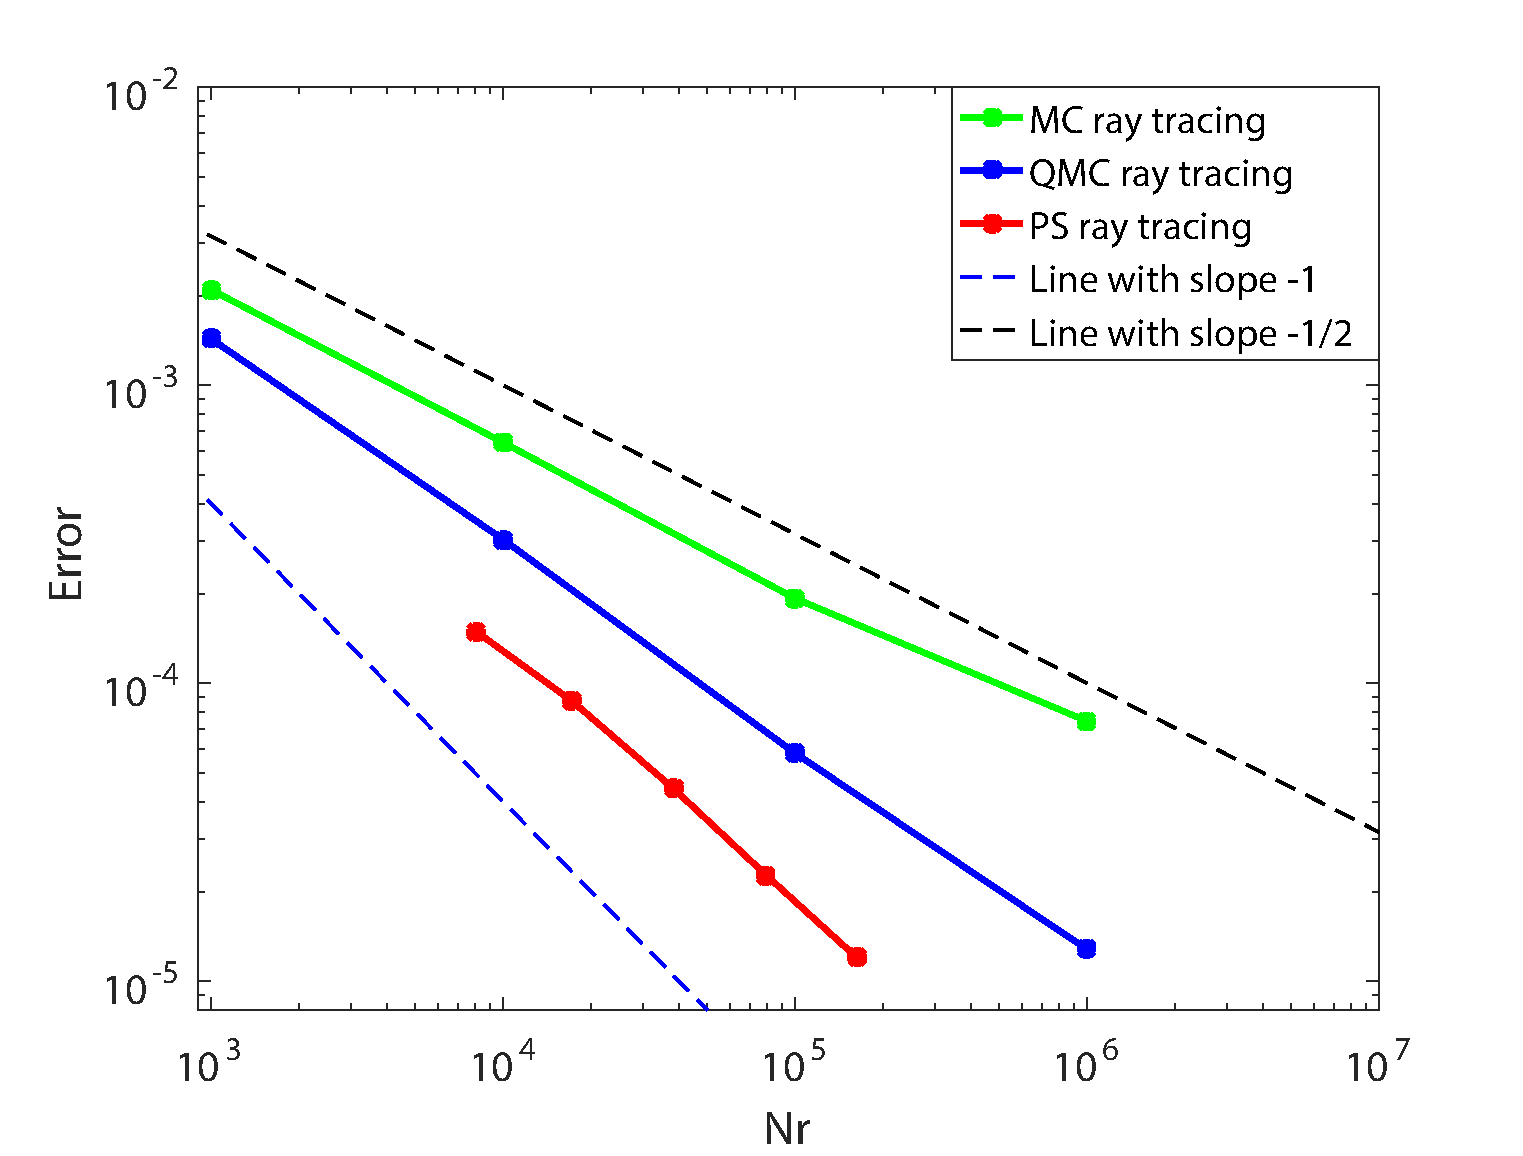
\includegraphics[width= 7cm]{error_tir_triangulation}
  \caption{\textbf{Error as a function of the number of rays} The PS intensity $\hat{I}_{\textrm{PS}}$ is computed using PS ray tracing with around $1.62\cdot 10^5$ rays. The reference intensity $\hat{I}_{\textrm{ref}}$ is obtained by QMC ray tracing with $10^7$ rays.}
  \label{fig:error_tir_triangulation}
\end{figure}
\\ \indent Finally, in order to show the advantages of PS ray tracing in terms of the computational time, in Figure \ref{fig:error_tir_triangulation_time} we provide an error convergence as a function of the CPU-time for MC, QMC and PS raytracing. The choice of the colours is consistent with Figure \ref{fig:intensity_tir_triangulation}.
\begin{figure}[ht]
  \center
  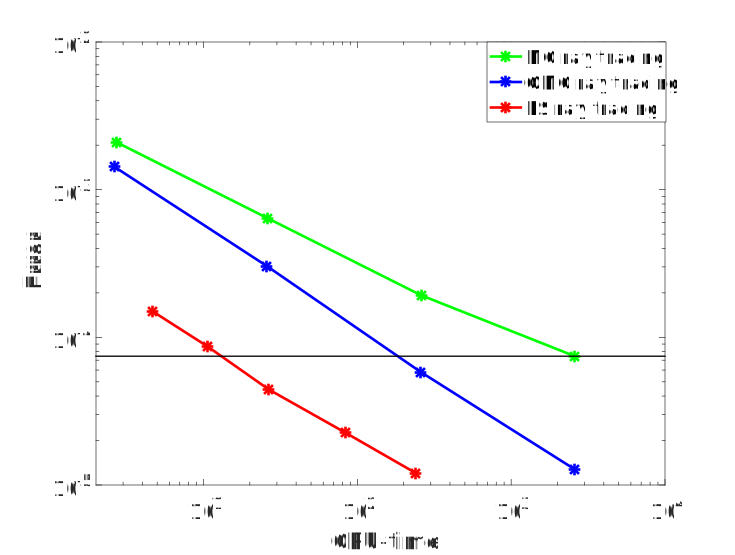
\includegraphics[width= 7cm]{error_tir_triangulation_time}
  \caption{\textbf{Error as a function of the CPU-time} The PS intensity $\hat{I}_{\textrm{PS}}$ is computed using PS ray tracing with around $1.62\cdot 10^5$ rays. The reference intensity $\hat{I}_{\textrm{ref}}$ is obtained by QMC ray tracing with $10^7$ rays.}
  \label{fig:error_tir_triangulation_time}
\end{figure}
% Discussion
\\ \indent To summarize, the results shown in Figures \ref{fig:error_tir_triangulation} and \ref{fig:error_tir_triangulation_time} are reported in Tables \ref{tab:ps_error_triangulation} and  \ref{tab:qmc_error_triangulation}.
\begin{table}[ht] \label{tab:table_tir_triangulation}
\centering
\caption{\bf Errors of the PS intensity}
\begin{tabular}{lllll}
 \hline   $\varepsilon_{\variabile{q}}^{\textrm{max}} $  & $\nrays$ & Etendue & PS error & CPU-time (sec.) \\
  \hline 
 $0.05$ & $3\,547$   & $7.50$   &  $1.75\cdot10^{-4}$ & $1.98$\\
$0.025$  & $8\,055$    & $7.61$    & $1.49\cdot 10^{-4}$ & $4.69$ \\
$0.125$  & $17\,300$    & $7.69$  & $8.68\cdot 10^{-5}$ & $10.61$\\
 $6.3 \cdot 10^{-3}$  & $38\,300$  & $7.73$   & $4.43\cdot 10^{-5}$ & $26.56$\\
 $3.1 \cdot 10^{-3}$ & $79\,600$  & $7.75$    & $2.27\cdot 10^{-5}$ & $83,21$\\
$1.6 \cdot 10^{-3}$ & $162\,300$  & $7.76$    & $1.20\cdot 10^{-5}$ & $240.53$\\
 \hline
 \end{tabular}
 \label{tab:ps_error_triangulation}
 \end{table}
\begin{table}[h!] \label{tab:table_tir_triangulation}
\centering
\caption{\bf Errors of the MC intensity and QMC intensity}
\begin{tabular}{lllll}
 \hline  $\nrays$\;  & MC error & QMC error & CPU-(MC)time (sec.) & CPU-(QMC)time (sec.)\\
  \hline 
 $10^3$ & $2.09\cdot 10^{-3}$  & $1.43\cdot10^{-3}$  & $2.73$  & $2.63$  \\
$10^4$  & $6.42\cdot 10^{-4}$  & $3.03\cdot 10^{-4}$  & $25.98$  & $25.84$   \\
$10^5$  & $1.92\cdot 10^{-4}$  & $5.82\cdot 10^{-5}$  & $259.92$  & $258.28$  \\
 $10^6$  & $7.45\cdot 10^{-5}$  & $1.28\cdot 10^{-5}$  & $2585.83$ & $2482.67$  \\
 \hline
 \end{tabular}
 \label{tab:qmc_error_triangulation}
 \end{table}



\section{A Parabolic reflector}
% Intensity 
% Error

\section{The Compound Parabolic Concentrator (CPC)}